\documentclass[11pt]{article}
\usepackage[margin=1in]{geometry}
\usepackage{amsmath,amssymb,graphicx,booktabs,hyperref,microtype,tikz}
\usetikzlibrary{matrix}
\usepackage[T1]{fontenc}
\hypersetup{colorlinks=true,linkcolor=black,urlcolor=blue}
\title{Library-free Q1 deconvolution of Sciex ZT scanning-DIA\\ \large A technical note, feasibility stage}
\author{Pioneer / ZT branch \texttt{feat/zt-scanning-v2}}
\date{18 September 2026}
\begin{document}\maketitle

\section{What the instrument records}
A ZT scanning acquisition sweeps a quadrupole window of nominal width $W$ (5\,Da here) continuously across the precursor range while the TOF records. The file stores the sweep as a lattice of \emph{bins}: one MS2 spectrum per Q1 step $S$ (1.02\,Da on the 5\,Da method, 496 bins per cycle from 393 to 899\,m/z). A bin at centre $q$ contains the fragments of every precursor whose transmission at $q$ is non-zero, each weighted by that transmission. We measured the transmission profile per file from the deconvolved weights of confident precursors: it is a symmetric triangle in Q1 offset $\Delta$,
\[
T(\Delta)=\max\!\left(0,\;1-\frac{|\Delta|}{h}\right),\qquad h\approx 6.5\text{ Da on every 5 Da method}\;(h/S\approx 6.4\text{--}6.6),
\]
so a precursor appears in $2k+1=13$ consecutive bins of one cycle, with its apex at the isotope centre of mass rather than at the monoisotopic m/z.

Pioneer currently handles this inside the search: candidates are expanded to all 13 bins, each bin is deconvolved separately, and the per-bin weights are collapsed to one meta-scan value per precursor per cycle. That works (96--108\% of DIA-NN direct on five methods) but it is a ZT-specific path through the whole engine.

\section{The idea}
Undo the sweep in the data before searching. Because every fragment's intensity along Q1 within a cycle is a sum of triangles centred on the precursors that produce it,
\[
y_r(j)=\sum_{s} T\!\big((j-s)\,S\big)\,x_r(s)+\varepsilon,
\]
where $r$ indexes fragment m/z, $j$ the recorded bin, and $x_r(s)$ is the fragment intensity that a hypothetical 1-Da isolation at slice $s$ would have produced. Given $T$, recovering $x_r(\cdot)$ from $y_r(\cdot)$ is a one-dimensional non-negative deconvolution per fragment row, independent of any spectral library. The result is a conventional narrow-window DIA file (one spectrum per 1-Da slice, isolation width $S$) that any engine searches without ZT machinery. The idea has literature roots in overlapping-window DIA demultiplexing (Amodei et al., JASMS 2019; the MSX demultiplexing of Egertson et al., Nat.\ Methods 2013, both implemented in msconvert). The ZT case is better conditioned than those: 13 overlapping measurements per slice instead of 2, and a measured, non-uniform kernel.

\section{The data support the model}
Figure~\ref{fig:streaks} shows a 2-Da fragment window of one dense cycle (RT 7.0 min) against Q1 centre. Every fragment is a horizontal streak $\approx$13 bins long, and the intensity profiles along Q1 of the strongest rows are clean triangles. The three strongest rows (613.86, 613.36, 612.32) peak at the same Q1 position: one precursor's unfragmented monoisotope and M+1 (charge 2, spacing 0.50 Da) and a fragment. Small bumps on the 613.325/613.825 rows near Q1 585 are a second precursor's isotopes sharing those fragment rows --- the overlap the deconvolution must separate. Adjacent bins agree on top peaks to 3 ppm (median), and the fraction of a bin's peaks found in bin $+1,+2,+3,+6$ is 72, 56, 43, 20\% --- the triangle seen from the fragment side.

\begin{figure}[h]\centering\includegraphics[width=0.9\textwidth]{q1_streaks_cycle382.png}
\caption{Top: fragment m/z 612--614 versus Q1 centre, cycle 382 (RT 7.01 min), 5 mDa grid, $\sigma$=1 bin smoothing, log colour. Bottom: Q1 profiles of the six strongest rows.}\label{fig:streaks}\end{figure}

\section{Algorithm}
Per cycle, on the $n_b$ MS2 bins of the ramp:
\begin{enumerate}
\item \textbf{Grid.} Bin each spectrum on a fixed m/z axis of step $g$ (5 mDa, i.e.\ 8 ppm at 600; the instrument's bin-to-bin jitter is 2--3 ppm). Keep, per (row, bin), $\sum \text{int}\cdot m/z$ and $\sum\text{int}$ so peak m/z can be recovered at instrument precision.
\item \textbf{Smooth in m/z.} Gaussian, $\sigma=1$ grid step, $\pm3$ steps. This repairs the peaks the jitter splits across two rows (Fig.~\ref{fig:grid}); $\sigma=2$ begins to merge neighbouring rows, and a 20 mDa grid without smoothing looks like 5 mDa with $\sigma=2$.
\item \textbf{Deconvolve along Q1}, one row at a time. Unknowns $x_r(s)$ for slices $s=1\ldots n_b+2k$ (the ramp plus $k$ slices beyond each end, so edge bins are explained). Design matrix $A_{js}=T\big((j-(s-k))S\big)$, banded of width $2k+1$. Solve $\min_{x\ge0}\|Ax-y\|^2$ by projected coordinate descent: for each slice, the exact 1-D minimiser $x_s\leftarrow\max(0,\,x_s+\langle a_s,r\rangle/\|a_s\|^2)$ with the residual $r$ updated in place; stop when the largest change in a sweep is below $10^{-3}$ of the row's peak intensity, or after 100 sweeps. Only Q1 segments where the row has signal are swept (a run of non-zero bins $[a,b]$ involves slices $a\ldots b+2k$ only), which is what makes the per-cycle cost tolerable. No regularisation beyond non-negativity. Section~\ref{sec:matrix} shows the system in matrix form with a worked example.
\item \textbf{Emit.} For slice $s$, one MS2 spectrum: every row with $x_r(s)\ge$ a floor (20 counts) becomes a peak with intensity $x_r(s)$ and m/z the intensity-weighted mean of the raw peak m/z in the row over bins $s\pm1$. Precursor m/z = bin centre, isolation width = $S$. MS1 scans pass through. Output uses Pioneer's Arrow schema.
\end{enumerate}
Only $h$ (equivalently $h/S$) is a parameter; it is measured from the file by the quad-tuning fit, and could be read from the streak widths themselves to keep the converter fully self-contained.

\begin{figure}[h]\centering\includegraphics[width=0.9\textwidth]{q1_heatmap_zoom_cycle382.png}
\caption{Fragment m/z 600--620 versus Q1 centre for the same cycle under four grid/smoothing settings.}\label{fig:grid}\end{figure}


\section{The deconvolution in matrix form, with a worked example}\label{sec:matrix}
Take one fragment row $r$ and drop the subscript. The recorded intensities down the Q1 ramp form a vector $y\in\mathbb{R}^{n_b}$, the unknown slice intensities a vector $x\in\mathbb{R}^{n_b+2k}_{\ge0}$, and
\[
y = A\,x,\qquad A_{js}=T\big((j-s')S\big),\; s'=s-k,
\]
so column $s$ of $A$ is the triangle a unit-intensity precursor at slice $s$ would leave across the bins, and row $j$ of $A$ lists which slices reach bin $j$ and with what weight. $A$ is banded: each column has $2k+1$ non-zeros, each row $2k+1$ non-zeros, and adjacent columns are shifted copies of one another. The $k$ extra slices at each end let a precursor sitting just outside the ramp explain the partial triangle it leaves at the edge.

\paragraph{Small example.} To keep the matrices readable use a triangle of half-base $h=2$ bins, so $T(-1)=T(1)=\tfrac12$, $T(0)=1$, and $k=1$: seven recorded bins $j=1\ldots7$, nine slices $s=0\ldots8$, and slice $s$ peaks at bin $s$.
\[
\underbrace{\begin{pmatrix}0\\50\\100\\70\\40\\20\\0\end{pmatrix}}_{y}
=
\underbrace{\begin{pmatrix}
\tfrac12&1&\tfrac12&\cdot&\cdot&\cdot&\cdot&\cdot&\cdot\\
\cdot&\tfrac12&1&\tfrac12&\cdot&\cdot&\cdot&\cdot&\cdot\\
\cdot&\cdot&\tfrac12&1&\tfrac12&\cdot&\cdot&\cdot&\cdot\\
\cdot&\cdot&\cdot&\tfrac12&1&\tfrac12&\cdot&\cdot&\cdot\\
\cdot&\cdot&\cdot&\cdot&\tfrac12&1&\tfrac12&\cdot&\cdot\\
\cdot&\cdot&\cdot&\cdot&\cdot&\tfrac12&1&\tfrac12&\cdot\\
\cdot&\cdot&\cdot&\cdot&\cdot&\cdot&\tfrac12&1&\tfrac12
\end{pmatrix}}_{A\;(7\times9)}
\underbrace{\begin{pmatrix}0\\0\\0\\100\\0\\40\\0\\0\\0\end{pmatrix}}_{x\;(\text{slices }0\ldots8)}
\]
The right-hand side is two precursors that share this fragment: intensity 100 at slice 3 and 40 at slice 5. Their triangles overlap at bin 4 ($50+20=70$), and the sum $y$ is a single hump with a shoulder, not two peaks (Fig.~\ref{fig:toy}). That is exactly the case a local-maximum (centroid) rule cannot separate: bin 5 (40) sits between 70 and 20 and is not a local maximum, so centroiding reports one precursor at slice 3 with a biased intensity. The least-squares solution does separate them because the shoulder is inconsistent with a single triangle.

\begin{figure}[h]\centering
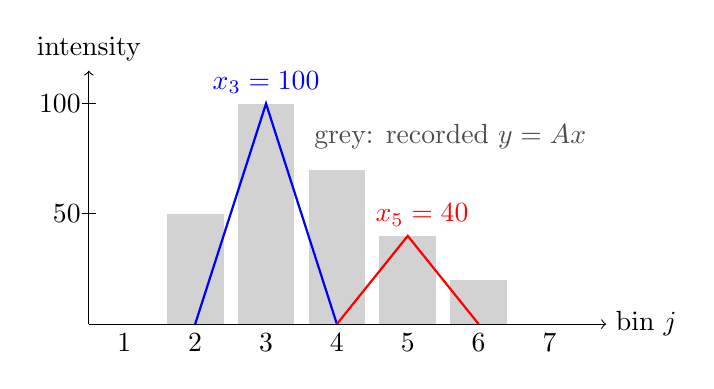
\begin{tikzpicture}[x=0.9cm,y=0.028cm]
\foreach \j/\v in {1/0,2/50,3/100,4/70,5/40,6/20,7/0}{\fill[gray!35] (\j-0.4,0) rectangle (\j+0.4,\v);}
\draw[thick,blue] (2,0)--(3,100)--(4,0); \draw[thick,red] (4,0)--(5,40)--(6,0);
\draw[->] (0.5,0)--(7.8,0) node[right]{bin $j$}; \draw[->] (0.5,0)--(0.5,115) node[above]{intensity};
\foreach \j in {1,...,7}{\node[below] at (\j,0) {\j};}
\foreach \v in {50,100}{\draw (0.4,\v)--(0.6,\v) node[left,xshift=-2pt]{\v};}
\node[blue,above] at (3,100) {$x_3=100$}; \node[red,above] at (5.2,40) {$x_5=40$};
\node[gray!60!black] at (5.6,85) {grey: recorded $y=Ax$};
\end{tikzpicture}
\caption{The toy row. Two overlapping triangles (blue, red) sum to the recorded profile (grey bars). The 40-count precursor is only a shoulder in $y$.}\label{fig:toy}
\end{figure}

\paragraph{Solving it.} $\min_{x\ge0}\|Ax-y\|^2$ by projected coordinate descent keeps a residual $r=y-Ax$ (initially $r=y$, $x=0$) and visits the slices in order. For slice $s$ with column $a_s$, the exact one-dimensional minimiser is
\[
x_s \leftarrow \max\!\Big(0,\;x_s+\frac{\langle a_s,r\rangle}{\|a_s\|^2}\Big),\qquad r\leftarrow r-a_s\,(x_s^{\text{new}}-x_s^{\text{old}}),
\]
with $\|a_s\|^2=1.5$ for interior slices and $1.25$, $0.25$ at the ends. The first sweep, slice by slice:
\begin{center}\small\begin{tabular}{crrrl}\toprule
$s$ & $\langle a_s,r\rangle$ & $\|a_s\|^2$ & $x_s$ & residual $r$ after the update\\\midrule
0 & 0.0 & 0.25 & 0.0 & $(0,50,100,70,40,20,0)$\\
1 & 25.0 & 1.25 & 20.0 & $(-20,40,100,70,40,20,0)$\\
2 & 80.0 & 1.50 & 53.3 & $(-46.7,-13.3,73.3,70,40,20,0)$\\
3 & 101.7 & 1.50 & 67.8 & $(-46.7,-47.2,5.6,36.1,40,20,0)$\\
4 & 58.9 & 1.50 & 39.3 & $(-46.7,-47.2,-14.1,-3.1,20.4,20,0)$\\
5 & 28.8 & 1.50 & 19.2 & $(-46.7,-47.2,-14.1,-12.7,1.2,10.4,0)$\\
6 & 11.0 & 1.50 & 7.3 & $(-46.7,-47.2,-14.1,-12.7,-2.5,3.1,-3.7)$\\
7 & $-2.1$ & 1.25 & 0.0 & unchanged (clamped at zero)\\
8 & $-1.8$ & 0.25 & 0.0 & unchanged\\\bottomrule
\end{tabular}\end{center}
After one sweep the mass is smeared over slices 1--6 because each slice greedily explained what was left. Later sweeps see the negative residual at bins 1--2, pull slices 1 and 2 back toward zero, and push the mass into slices 3 and 5:
\begin{center}\small\begin{tabular}{crrrrrrrrrr}\toprule
sweep & $x_0$ & $x_1$ & $x_2$ & $x_3$ & $x_4$ & $x_5$ & $x_6$ & $x_7$ & $x_8$ & $\|r\|$\\\midrule
1 & 0 & 20.0 & 53.3 & 67.8 & 39.3 & 19.2 & 7.3 & 0 & 0 & 69.3\\
2 & 0 & 0 & 14.9 & 67.3 & 31.9 & 19.3 & 8.5 & 0 & 0 & 13.9\\
5 & 0 & 0 & 12.6 & 77.1 & 24.6 & 21.9 & 8.0 & 0 & 0 & 9.8\\
10 & 0 & 0 & 7.8 & 85.0 & 16.9 & 27.1 & 5.8 & 0 & 0 & 6.5\\
20 & 0 & 0 & 3.7 & 92.8 & 8.2 & 33.7 & 2.8 & 0 & 0 & 3.1\\
46 & 0 & 0 & 0.6 & 98.9 & 1.2 & 39.1 & 0.4 & 0 & 0 & 0.5\\\bottomrule
\end{tabular}\end{center}
The stop test (largest change below $10^{-3}$ of the row's peak) fires at sweep 46 with $x_3=98.9$, $x_5=39.1$ against the truth 100 and 40. Two things are visible here that carry over to the real problem. First, convergence is slow because adjacent columns of $A$ are nearly parallel (their triangles overlap heavily), so the solver moves mass between neighbouring slices one small step at a time; with the real $k=6$ the columns are even more alike, which is why 100 sweeps is the cap. Second, the answer is not perfectly sparse: a few counts leak into the slices adjacent to each true one (0.6, 1.2, 0.4 above). The emit step's intensity floor removes most of that leakage, and the centroid variant of the converter avoids it entirely at the price of the shoulder case shown in Fig.~\ref{fig:toy}.

\paragraph{The real problem.} Per cycle the same solve runs for every active fragment row, with $n_b=496$ bins, $508$ slices, and a triangle of half-base $h/S=6.49$ bins ($13$ non-zeros per column). Rows are independent, so they run in parallel, and each row is only swept over the Q1 segments where it has signal.

\section{Feasibility measurements}
Region: RT 7.0$\pm$0.015 min (2 cycles), Q1 580--640, fragments 300--900; ground truth = 51 precursors Pioneer identified there, their top-8 library fragments (701 fragment rows). ``Own slice'' = the bin nearest the precursor's isotope centre of mass. \emph{Local concentration} = mass within $\pm1$ slice of the own slice, as a fraction of the mass within $\pm6$; for a clean triangle the raw value is 0.41 by geometry, and a perfect deconvolution gives 1.

\begin{center}\begin{tabular}{lrrrrr}\toprule
fragment ranks & rows & raw median & deconvolved median & deconvolved p25 & $\ge$0.8 \\ \midrule
1--3 & 206 & 0.43 & \textbf{0.90} & 0.40 & 57\% \\
4--8 & 354 & 0.38 & 0.61 & 0.00 & 38\% \\
all  & 701 & 0.39 & 0.64 & 0.00 & 42\% \\ \bottomrule
\end{tabular}\end{center}

Three examples from one precursor (588.306, z=2), raw profile $y$ over own slice $\pm6$ and deconvolved $x$:
\begin{center}\small\begin{tabular}{lll}\toprule
fragment & raw $y$ & deconvolved $x$ \\ \midrule
784.468 (rank 3) & 0 38 753 1419 1484 2052 2270 2073 1593 1332 600 0 0 & 0 0 0 0 0 28 \textbf{2233} 0 0 0 0 0 0 \\
392.145 (rank 5) & 80 443 1006 1338 1769 2325 2545 2012 1844 1423 1062 608 0 & 0 0 0 0 0 218 \textbf{2248} 0 118 0 0 0 0 \\
656.409 (rank 1) & 4642 6049 7636 8116 8555 10262 9773 9972 8076 6589 4632 1647 197 & 2345 1158 291 0 0 4015 2402 4575 0 0 0 0 0 \\ \bottomrule
\end{tabular}\end{center}
The first two collapse an 11-bin triangle to a single slice. The third is two overlapping triangles in the raw data and the deconvolution splits it into two components six slices apart: two precursors sharing a fragment m/z, separated.

Sparsity: a deconvolved slice has 0.29$\times$ the nonzero rows of a raw bin (31,000 $\to$ 9,100), i.e.\ the 13-fold spreading is largely undone.

\section{What is not yet known}
\begin{itemize}
\item The end-to-end test: a 1-minute window (56 cycles, RT 6.5--7.5) is being converted; it will be searched as ordinary DIA (scanning-quad off) against the same window searched through the ZT path, comparing precursor counts and overlap. This is the number that decides whether to build the converter properly.
\item Low-rank fragments deconvolve noisily (p25 = 0); whether this costs identifications or is absorbed by scoring is what the search will show.
\item Noise: NNLS with a 13-wide kernel can spread a weak streak over neighbouring slices; a mild ridge or a sparsity prior may help, untested.
\item Speed: the current solver sweeps all 508 slices of every active row (320,000 rows per cycle); restricting each row to the slices near its signal is an order-of-magnitude saving with identical results.
\item Quant: the deconvolved slice intensity is the least-squares abundance under the profile, the same estimator the matched-filter meta-scan reduction uses, so quant should carry over; unverified.
\end{itemize}
\end{document}
